\documentclass[aspectratio=169,10pt]{beamer}
\usetheme{Madrid}
\usecolortheme{default}
\usepackage[spanish]{babel}
\usepackage[T1]{fontenc}
\usepackage{graphicx}
\usepackage{hyperref}
\usepackage{booktabs}
\usepackage{xcolor}
\usepackage{tikz}
\usepackage{listings}
\usepackage{caption}
\usepackage{multicol}
\usepackage[absolute,overlay]{textpos}

% Configuración de colores
\definecolor{darkred}{rgb}{0.8, 0, 0}
\definecolor{darkblue}{rgb}{0, 0, 0.6}
\definecolor{darkgreen}{rgb}{0, 0.5, 0}
\setbeamercolor{title}{fg=white,bg=darkred}
\setbeamercolor{frametitle}{fg=white,bg=darkred}
\setbeamercolor{block title}{fg=white,bg=darkred}

% Reducir espaciado de bloques
\setbeamertemplate{blocks}[rounded][shadow=false]
\addtobeamertemplate{block begin}{\setlength{\parskip}{3pt}}{}
\addtobeamertemplate{block body}{\setlength{\parskip}{2pt}}{}

% Reducir espacios entre títulos de frame
\setbeamerfont{frametitle}{size=\large}
\setbeamertemplate{frametitle}{\insertframetitle\par\vskip-3pt}

% Configuración de código
\lstset{
    basicstyle=\tiny\ttfamily,
    breaklines=true,
    language=Python,
    showstringspaces=false,
    tabsize=2
}

% Reducir espaciado en listas
\usepackage{enumitem}
\setlist[itemize]{itemsep=2pt, topsep=2pt}
\setlist[enumerate]{itemsep=2pt, topsep=2pt}

% Eliminar autor del pie de página
\setbeamertemplate{footline}{%
  \hbox{%
    \begin{beamercolorbox}[wd=\paperwidth,ht=2.25ex,dp=1ex]{palette quaternary}%
      \hspace*{1em}
      \usebeamerfont{page number in head/foot}%
      \usebeamercolor[fg]{page number in head/foot}%
      \insertframenumber\hspace*{1em}
    \end{beamercolorbox}%
  }%
}

\title{Moderador Automático de Contenido en Videos}
\subtitle{Transcripción, Etiquetado y Clasificación de Contenido Inapropiado}
\author{
  \textbf{Grupo 4:}\\
  Koc Góngora, Luis Enrique\\
  Mancilla Antay, Alex Felipe\\
  Melendez Garcia, Herbert Antonio\\
  Paitan Cano, Dennis Jack
}
\institute{
Maestría en Inteligencia Artificial\\
Universidad Nacional de Ingeniería (UNI)\\
Procesamiento de Lenguaje Natural
}
\date{Semestre 2026-1}

\begin{document}

% ==================== PORTADA ====================
\begin{frame}
  \titlepage
\end{frame}

% ==================== SLIDE 2: PROBLEMÁTICA ====================
\begin{frame}
  \frametitle{Problemática: Moderación de Contenido en Plataformas de Video}
  
  \begin{block}{Desafío Global}
    \begin{itemize}
      \item Plataformas como YouTube, TikTok generan \textbf{500+ horas de video por minuto}
      \item Contenido en idioma español crece exponencialmente en creadores peruanos
      \item Moderación manual es \textbf{costosa, lenta e inconsistente}
    \end{itemize}
  \end{block}
  
  \begin{block}{Brecha de Investigación}
    \begin{enumerate}
      \item No existen soluciones locales para moderación de contenido en español (Perú)
      \item Modelos LLM externos = privacidad limitada y costos operacionales altos
      \item \textbf{Propuesta:} Sistema end-to-end local para transcripción y clasificación automática
    \end{enumerate}
  \end{block}

  \begin{block}{Objetivo}
    Desarrollar un moderador automático que funcione \textbf{100\% localmente} sin depender de APIs externas
  \end{block}
\end{frame}

% ==================== SLIDE 3: ARQUITECTURA GENERAL ====================
\begin{frame}
  \frametitle{Arquitectura General del Sistema}
  
  \begin{columns}[T]
    \column{0.75\textwidth}
      \centering
      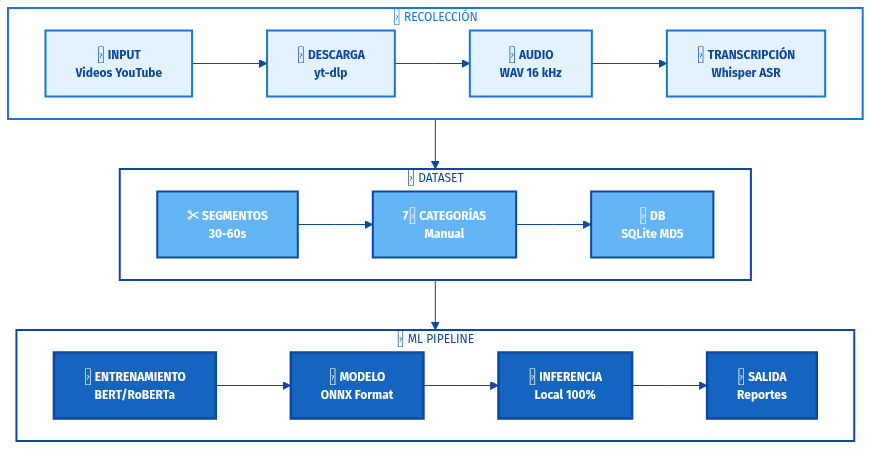
\includegraphics[width=\textwidth,height=5cm,keepaspectratio]{arquitectura_sistema.png}
    
    \column{0.25\textwidth}
      \vspace{0.5cm}
      \small
      \begin{block}{Pipeline}
        \tiny
        \begin{enumerate}[itemsep=1pt]
          \item Descarga de video (yt-dlp)
          \item Procesamiento audio
          \item Transcripción (Whisper)
          \item Segmentación
          \item Etiquetado manual
          \item Limpieza datos
          \item Entrenamiento
          \item Exportación (ONNX)
          \item Inferencia local
          \item Reportes
        \end{enumerate}
      \end{block}
  \end{columns}
\end{frame}

% ==================== SLIDE 4: PARTE A - CREACIÓN DE DATASET (1/4) ====================
\begin{frame}[fragile]
  \frametitle{A.1. Descarga de Audio desde YouTube}
  
  \begin{columns}[T]
    \column{0.7\textwidth}
      \begin{block}{Especificaciones Técnicas}
        \small
        \begin{itemize}
          \item \textbf{Duración:} 50--100 horas de audio ($\approx$ 1000 videos 5 min)
          \item \textbf{Framerate:} 16 kHz (estándar ASR)
          \item \textbf{Canales:} Política, Farándula, Comida, Viajes peruanos
          \item \textbf{Formato output:} WAV mono a 16kHz
        \end{itemize}
      \end{block}

      \begin{block}{Arquitectura Python}
        \small
        \begin{itemize}
          \item \textbf{Herramienta:} \texttt{yt-dlp} (descendiente youtube-dl)
          \item \textbf{Flujo:}
          \begin{enumerate}[itemsep=1.1pt]
            \item Scraping URLs de canales peruanos
            \item Descarga mejor calidad audio
            \item Conversión a WAV 16kHz mono
            \item Almacenamiento en carpetas categorizadas
          \end{enumerate}
          \item \textbf{Manejo errores:} Reintentos con backoff
          \item \textbf{Storage:} Carpetas por categoría/fecha
        \end{itemize}
      \end{block}
    
    \column{0.25\textwidth}
      \vspace{-0.3cm}
      \begin{block}{Pseudocódigo}
        \tiny
        \begin{lstlisting}[basicstyle=\tiny\ttfamily,breaklines=true]
import yt_dlp

ydl = yt_dlp.YoutubeDL({
  'format': 'bestaudio',
  'audio-format': 'wav',
  'audio-quality': '192',
  'quiet': False
})

for url in url_list:
  ydl.download([url])
        \end{lstlisting}
      \end{block}
  \end{columns}
\end{frame}

% ==================== SLIDE 5: PARTE A - TRANSCRIPCIÓN (2/4) ====================
\begin{frame}
  \frametitle{A.2. Transcripción Local con Modelos ASR}
  
  \begin{block}{Modelos Recomendados (Local) \cite{radford2022whisper}}
    \begin{itemize}
      \item \textbf{Whisper OpenAI (base/small):} $\sim$81M params, $\sim$1.5GB RAM, excelente en español
      \item \textbf{Wav2Vec2 Facebook:} $\sim$317M params, entrenado multilingüe
      \item \textbf{xlsr-wav2vec2-spanish:} Optimizado para español peruano
    \end{itemize}
  \end{block}

  \begin{block}{Justificación}
    \begin{itemize}
      \item \textbf{Whisper:} Robusto a ruido y acentos, mejor precisión en español
      \item \textbf{Wav2Vec2:} Menor consumo de memoria, inferencia rápida
      \item Todos ejecutables localmente en GPU modesta (RTX 3060+)
    \end{itemize}
  \end{block}

  \begin{block}{Métricas esperadas}
    WER (Word Error Rate) en español: 8--15\% para Whisper base
  \end{block}
\end{frame}

% ==================== SLIDE 6: PARTE A - ETIQUETADO (3/4) ====================
\begin{frame}
  \frametitle{A.3. Framework HTML para Etiquetado Manual}
  
  \begin{block}{Categorías de Moderación (7 etiquetas)}
    \begin{enumerate}
      \item \textbf{Lenguaje Inapropiado} (insultos, groserías)
      \item \textbf{Racismo/Discriminación} (xenofobia, prejuicio étnico)
      \item \textbf{Sexismo} (misoginia, discriminación de género)
      \item \textbf{Contenido Sexual Explícito} (referencias sexuales, acoso)
      \item \textbf{Violencia} (amenazas, incitación a violencia)
      \item \textbf{Desinformación/Odio} (fake news, incitación a odio)
      \item \textbf{Limpio} (sin violación de moderación)
    \end{enumerate}
  \end{block}

  \begin{block}{Interfaz Propuesta}
    HTML5 + JavaScript local: cargar chunks, selector de categoría (botones), persistencia en LocalStorage JSON
  \end{block}
\end{frame}

% ==================== SLIDE 7: PARTE A - DATASET INCREMENTAL (4/4) ====================
\begin{frame}
  \frametitle{A.4. Dataset Incremental y Limpieza}
  
  \begin{block}{Estructura Incremental}
    \begin{itemize}
      \item Base datos: \textbf{SQLite} (local, sin servidor)
      \item Schema: \texttt{(chunk\_id, texto, etiqueta, timestamp, hash\_MD5)}
      \item Hash MD5 del texto para detectar duplicados
    \end{itemize}
  \end{block}

  \begin{block}{Verificación de Consistencia}
    \begin{enumerate}
      \item Antes de insertar: verificar si chunk existe (por hash)
      \item Si duplicado: comparar etiqueta, reportar inconsistencias
      \item Versioning: mantener histórico de cambios
      \item Output limpio: JSON con balanceo de clases
    \end{enumerate}
  \end{block}

  \begin{block}{Resultado Final}
    Dataset de $\approx 5000$--$10000$ chunks etiquetados, balanceado, sin duplicados, listo para entrenamiento
  \end{block}
\end{frame}

% ==================== SLIDE 8: PARTE B - ENTRENAMIENTO ====================
\begin{frame}
  \frametitle{B. Entrenamiento: Comparativa de Modelos}
  
  \begin{block}{Propuesta: Ensemble de Modelos \cite{devlin2018bert}}
    \begin{enumerate}
      \item \textbf{BERT (Transformer):} Transfer learning, SOTA para clasificación
        \begin{itemize}
          \item Fine-tuning en dataset etiquetado
          \item Precisión esperada: 88--92\%
        \end{itemize}
      \item \textbf{SVM (Clásico):} Baseline robusto, menos datos necesarios
        \begin{itemize}
          \item Vectorización: TF-IDF + Word2Vec
          \item Precisión esperada: 75--82\%
        \end{itemize}
      \item \textbf{RoBERTa:} Mejora sobre BERT, mejor en toxicity detection \cite{liu2019roberta}
    \end{enumerate}
  \end{block}

  \begin{block}{Herramienta Recomendada}
    \textbf{Hugging Face Transformers} + PyTorch para Transformers; \textbf{scikit-learn} para SVM
  \end{block}
\end{frame}

% ==================== SLIDE 9: EVALUACIÓN ====================
\begin{frame}
  \frametitle{Evaluación de Modelos}
  
  \begin{block}{Métricas Propuestas}
    \begin{itemize}
      \item \textbf{Accuracy:} Métrica global
      \item \textbf{Precision/Recall:} Por categoría (especialmente clases raras)
      \item \textbf{F1-Score:} Balance entre precisión y recall
      \item \textbf{ROC-AUC:} Curva característica para categorías críticas
    \end{itemize}
  \end{block}

  \begin{block}{Validación}
    \begin{enumerate}
      \item Train: 70\% del dataset
      \item Validation: 15\%
      \item Test: 15\% (hold-out para evaluación final)
      \item Cross-validation: 5-fold para robustez
    \end{enumerate}
  \end{block}

  \begin{block}{Justificación \cite{bishop2006pattern}}
    Split 70--15--15 es estándar en NLP y ML
  \end{block}
\end{frame}

% ==================== SLIDE 10: PARTE C - FRAMEWORK DE PRODUCCIÓN ====================
\begin{frame}
  \frametitle{C. Framework de Producción e Inferencia}
  
  \begin{block}{Arquitectura}
    \begin{itemize}
      \item \textbf{Backend:} Flask/FastAPI (Python)
      \item \textbf{Modelos:} Cargados en memoria (ONNX para optimización)
      \item \textbf{Frontend:} Streamlit o Dashboard React simple
      \item \textbf{Base de datos:} SQLite (local)
    \end{itemize}
  \end{block}

  \begin{block}{Pipeline de Inferencia}
    \begin{enumerate}
      \item Input: URL de video o archivo de audio
      \item Descargar/procesar audio
      \item Transcripción con Whisper
      \item Segmentación en chunks (30--60 segundos)
      \item Predicción: pasar cada chunk por modelo BERT fine-tuned
      \item Output: JSON con predicciones y confianza
    \end{enumerate}
  \end{block}

  \begin{block}{Ventajas}
    \textbf{100\% local, sin dependencias externas, privacidad garantizada}
  \end{block}
\end{frame}

% ==================== SLIDE 11: CASOS DE USO ====================
\begin{frame}
  \frametitle{Casos de Uso y Beneficiarios}
  
  \begin{block}{Plataformas de Contenido}
    \begin{itemize}
      \item Creadores de YouTube/TikTok peruanos
      \item Moderación automática pre-publicación
      \item Análisis retrospectivo de contenido
    \end{itemize}
  \end{block}

  \begin{block}{Instituciones}
    \begin{itemize}
      \item Ministerios (monitoreo de desinformación)
      \item Universidades (investigación en NLP español)
      \item ONGs (detección de acoso/ciberabuso)
    \end{itemize}
  \end{block}

  \begin{block}{Impacto}
    Solución local, privacidad garantizada, adaptable a contexto peruano
  \end{block}
\end{frame}

% ==================== SLIDE 12: LIMITACIONES ====================
\begin{frame}
  \frametitle{Limitaciones y Trabajo Futuro}
  
  \begin{block}{Limitaciones Actuales}
    \begin{itemize}
      \item Dataset limitado ($\approx 5000$--$10000$ chunks)
      \item Requiere GPU para inferencia rápida
      \item Dependencia de calidad de transcripción Whisper
      \item Sesgo en categorías minoritarias
    \end{itemize}
  \end{block}

  \begin{block}{Mejoras Futuras}
    \begin{enumerate}
      \item Aumentar dataset a 50K+ chunks
      \item Fine-tuning de Whisper específico para español peruano
      \item Modelos multimodales (audio + video)
      \item Explainability (LIME/SHAP) para decisiones
      \item API REST completamente funcional
    \end{enumerate}
  \end{block}
\end{frame}

% ==================== SLIDE 13: CRONOGRAMA ====================
\begin{frame}
  \frametitle{Cronograma Propuesto}
  
  \begin{center}
    \begin{tabular}{l|c|c}
      \toprule
      \textbf{Fase} & \textbf{Duración} & \textbf{Mes} \\
      \midrule
      A.1 Descarga de datos & 1.5 semanas & Junio \\
      A.2 Transcripción ASR & 1.5 semanas & Junio \\
      A.3 Etiquetado manual & 3 semanas & Junio--Julio \\
      A.4 Dataset limpio & 1 semana & Julio \\
      \midrule
      B Entrenamiento & 2 semanas & Julio \\
      \midrule
      C Framework producción & 1.5 semanas & Julio \\
      \midrule
      Documentación + Demo & 1 semana & Julio \\
      \bottomrule
    \end{tabular}
  \end{center}

  \vspace{0.5cm}
  \textit{\small Total: $\sim$ 12 semanas de trabajo integrado}
\end{frame}

% ==================== SLIDE 14: REFERENCIAS BIBLIOGRÁFICAS ====================
\begin{frame}[allowframebreaks]
  \frametitle{Referencias Bibliográficas}
  
  \begin{thebibliography}{99}
  
    \bibitem[Radford et al., 2022]{radford2022whisper}
    Radford, A., Kim, J. W., Xu, T., Brockman, G., McLeavey, C., \& Sutskever, I. (2022).
    \newblock Robust Speech Recognition via Large-Scale Weak Supervision.
    \newblock \textit{arXiv preprint arXiv:2212.04356}.
    
    \bibitem[Devlin et al., 2018]{devlin2018bert}
    Devlin, J., Chang, M. W., Lee, K., \& Toutanova, K. (2018).
    \newblock BERT: Pre-training of Deep Bidirectional Transformers for Language Understanding.
    \newblock \textit{arXiv preprint arXiv:1810.04805}.
    
    \bibitem[Liu et al., 2019]{liu2019roberta}
    Liu, Y., Ott, M., Goyal, N., Du, J., Joshi, M., Chen, D., Levy, O., Lewis, M., Zettlemoyer, L., \& Stoyanov, V. (2019).
    \newblock RoBERTa: A Robustly Optimized BERT Pretraining Approach.
    \newblock \textit{arXiv preprint arXiv:1907.11692}.
    
    \bibitem[Bishop, 2006]{bishop2006pattern}
    Bishop, C. M. (2006).
    \newblock Pattern Recognition and Machine Learning.
    \newblock \textit{Springer Science+Business Media}.
    
    \bibitem[Pitsilis et al., 2018]{pitsilis2018detecting}
    Pitsilis, V., Ramampiaro, H., \& Langseth, H. (2018).
    \newblock Detecting Offensive Language in Tweets Using Deep Learning.
    \newblock \textit{arXiv preprint arXiv:1801.04354}.
    
    \bibitem[Ribeiro et al., 2020]{ribeiro2020beyond}
    Ribeiro, M. T., Wu, T., Guestrin, C., \& Singh, A. (2020).
    \newblock Beyond Accuracy: Behavioral Testing of NLP Models with CheckList.
    \newblock \textit{In Proceedings of the 58th Annual Meeting of the Association for Computational Linguistics}, 4902--4912.
    
  \end{thebibliography}
\end{frame}

\end{document}
